
\par $S = [2,4]$

\vskip 0.3in
\par $S_{alternativa^+} = [2,3]$ \qquad $S_{alternativa^-} = [0,1]$
\par $H(S_{alternativa^+}) = -\frac{2}{5} \log_2 \frac{2}{5}- \frac{3}{5} \log_2 \frac{3}{5} = 0.971$
\par $H(S_{alternativa^-}) = -\frac{0}{1} \log_2 \frac{0}{1}- \frac{1}{1} \log_2 \frac{1}{1} = 0.000$
\par $Ganho(S, S_{alternativa}) = 0.918-\frac{5}{6} * 0.971-\frac{1}{6} * 0.000 = 0.109$

\vskip 0.3in
\par $S_{bar^+} = [1,2]$ \qquad $S_{bar^-} = [1,2]$
\par $H(S_{bar^+}) = -\frac{1}{3} \log_2 \frac{1}{3}- \frac{2}{3} \log_2 \frac{2}{3} = 0.918$
\par $H(S_{bar^-}) = -\frac{1}{3} \log_2 \frac{1}{3}- \frac{2}{3} \log_2 \frac{2}{3} = 0.918$
\par $Ganho(S, S_{bar}) = 0.918-\frac{3}{6} * 0.918-\frac{3}{6} * 0.918 = 0.000$

\vskip 1in
\par $S_{fimSemana^+} = [2,3]$ \qquad $S_{fimSemana^-} = [0,1]$
\par $H(S_{fimSemana^+}) = -\frac{2}{5} \log_2 \frac{2}{5}- \frac{3}{5} \log_2 \frac{3}{5} = 0.971$
\par $H(S_{fimSemana^-}) = -\frac{0}{1} \log_2 \frac{0}{1}- \frac{1}{1} \log_2 \frac{1}{1} = 0.000$
\par $Ganho(S, S_{fimSemana}) = 0.918-\frac{5}{6} * 0.971-\frac{1}{6} * 0.000 = 0.109$

\vskip 0.3in
\par $S_{fome^+} = [2,2]$ \qquad   $S_{fome^-} = [0,2]$
\par $Ganho(S_{cheio}, S_{fome}) = 0.251$

\vskip 0.3in
\par $S_{preço^{\$}} = [2,2]$ \qquad $S_{preço^{\$\$\$}} = [0,2]$
\par $H(S_{preço^{\$}}) = -\frac{2}{4} \log_2 \frac{2}{4}- \frac{2}{4} \log_2 \frac{2}{4} = 1.000$
\par $H(S_{preço^{\$\$\$}}) = -\frac{0}{2} \log_2 \frac{0}{2}- \frac{2}{2} \log_2 \frac{2}{2} = 0.000$
\par $Ganho(S, S_{preço}) = 0.918-\frac{4}{6} * 1.000-\frac{2}{6} * 0.000 = 0.251$

\vskip 0.3in
\par $S_{chuva^+} = [1,1]$ \qquad $S_{chuva^-} = [1,3]$
\par $H(S_{chuva^+}) = -\frac{1}{2} \log_2 \frac{1}{2}- \frac{1}{2} \log_2 \frac{1}{2} = 1.000$
\par $H(S_{chuva^-}) = -\frac{1}{4} \log_2 \frac{1}{4}- \frac{3}{4} \log_2 \frac{3}{4} = 0.811$
\par $Ganho(S, S_{chuva}) = 0.918-\frac{2}{6} * 1.000-\frac{4}{6} * 0.811 = 0.044$

\vskip 0.3in
\par $S_{reserva^+} = [0,2]$ \qquad $S_{reserva^-} = [2,2]$
\par $H(S_{reserva^+}) = -\frac{0}{2} \log_2 \frac{0}{2}- \frac{2}{2} \log_2 \frac{2}{2} = 0.000$
\par $H(S_{reserva^-}) = -\frac{2}{4} \log_2 \frac{2}{4}- \frac{2}{4} \log_2 \frac{2}{4} = 1.000$
\par $Ganho(S, S_{reserva}) = 0.918-\frac{2}{6} * 0.000-\frac{4}{6} * 1.000 = 0.251$

\vskip 0.3in
\par $S_{tipo^{Francês}} = [0,1]$ \qquad $S_{tipo^{Tainlandês}} = [1,1]$\par $S_{tipo^{Italiano}} = [0,1]$ \qquad $S_{tipo^{Hamburger}} = [1,1]$
\par $H(S_{tipo^{Francês}}) = -\frac{0}{1} \log_2 \frac{0}{1}- \frac{1}{1} \log_2 \frac{1}{1} = 0.000$
\par $H(S_{tipo^{Tainlandês}}) = -\frac{1}{2} \log_2 \frac{1}{2}- \frac{1}{2} \log_2 \frac{1}{2} = 1.000$
\par $H(S_{tipo^{Italiano}}) = -\frac{0}{1} \log_2 \frac{0}{1}- \frac{1}{1} \log_2 \frac{1}{1} = 0.000$
\par $H(S_{tipo^{Hamburger}}) = -\frac{1}{2} \log_2 \frac{1}{2}- \frac{1}{2} \log_2 \frac{1}{2} = 1.000$
\par $Ganho(S, S_{tipo}) = 0.918-\frac{1}{6} * 0.000-\frac{2}{6} * 1.000-\frac{1}{6} * 0.000-\frac{2}{6} * 1.000 = 0.251$

\vskip 0.3in
\par $S_{tempoEspera^{10-30}} = [1,1]$ \qquad $S_{tempoEspera^{30-60}} = [1,1]$ \qquad $S_{tempoEspera^{>60}} = [0,2]$
\par $H(S_{tempoEspera^{10-30}}) = -\frac{1}{2} \log_2 \frac{1}{2}- \frac{1}{2} \log_2 \frac{1}{2} = 1.000$
\par $H(S_{tempoEspera^{30-60}}) = -\frac{1}{2} \log_2 \frac{1}{2}- \frac{1}{2} \log_2 \frac{1}{2} = 1.000$
\par $H(S_{tempoEspera^{>60}}) = -\frac{0}{2} \log_2 \frac{0}{2}- \frac{2}{2} \log_2 \frac{2}{2} = 0.000$
\par $Ganho(S, S_{tempoEspera}) = 0.918-\frac{2}{6} * 1.000-\frac{2}{6} * 1.000-\frac{2}{6} * 0.000 = 0.251$

\vskip 0.4in
\hfil
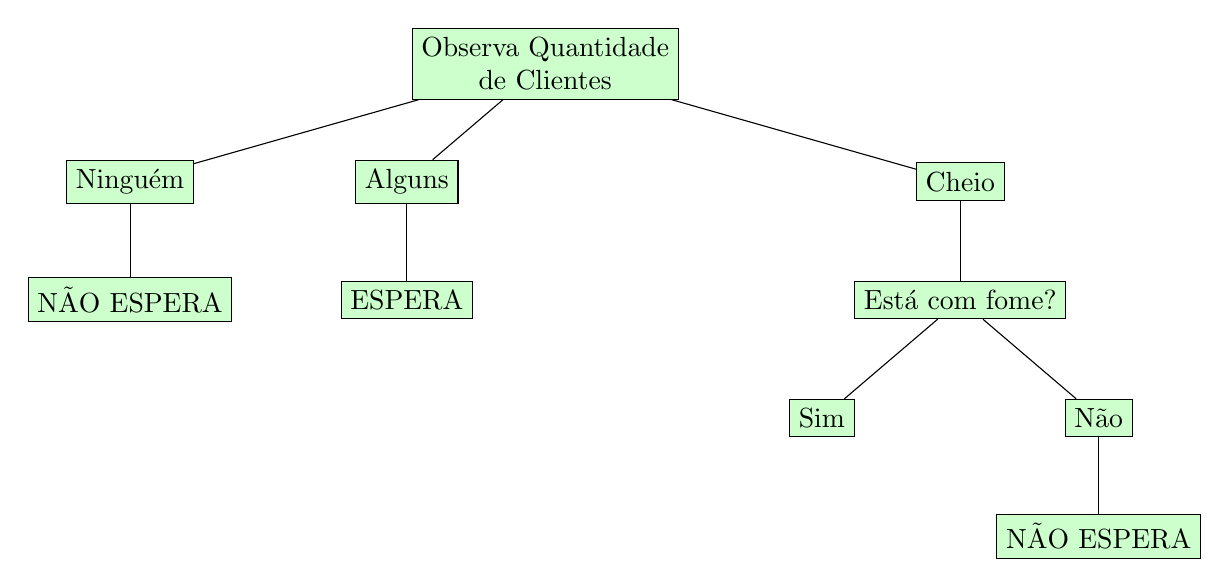
\begin{tikzpicture}[sibling distance=10em,
    every node/.style = {shape=rectangle, 
      draw, align=center,
      top color=green!20, bottom color=green!20}]]
    \node {Observa Quantidade \\ de Clientes}
        child { node {Ninguém} child { node {NÃO ESPERA}  } }
        child { node {Alguns} child { node {ESPERA}  } }
        child [missing]
        child { node {Cheio} child { 
            node {Está com fome?} child { node {Sim}  } child { node {Não} child { node {NÃO ESPERA}  }  }
            }
        };
  \end{tikzpicture}